\documentclass[border=3pt]{standalone}
\usepackage{fontspec}
\setmainfont{Times New Roman}
\usepackage{pgfplots}
\pgfplotsset{compat=1.18}
\usetikzlibrary{arrows.meta,calc,positioning,shapes.geometric}
\definecolor{forest}{HTML}{346E57}
\definecolor{sage}{HTML}{E8EFEA}
\definecolor{clay}{HTML}{B77E60}
\definecolor{gray}{HTML}{718078}
\definecolor{rule}{HTML}{B7C3BA}
\definecolor{ink}{HTML}{000000}
\begin{document}
\hyphenpenalty=10000\exhyphenpenalty=10000
\fontsize{10}{12}\selectfont
\renewcommand{\small}{\fontsize{9}{11}\selectfont}
\renewcommand{\scriptsize}{\fontsize{8}{10}\selectfont}
\resizebox{16cm}{!}{%
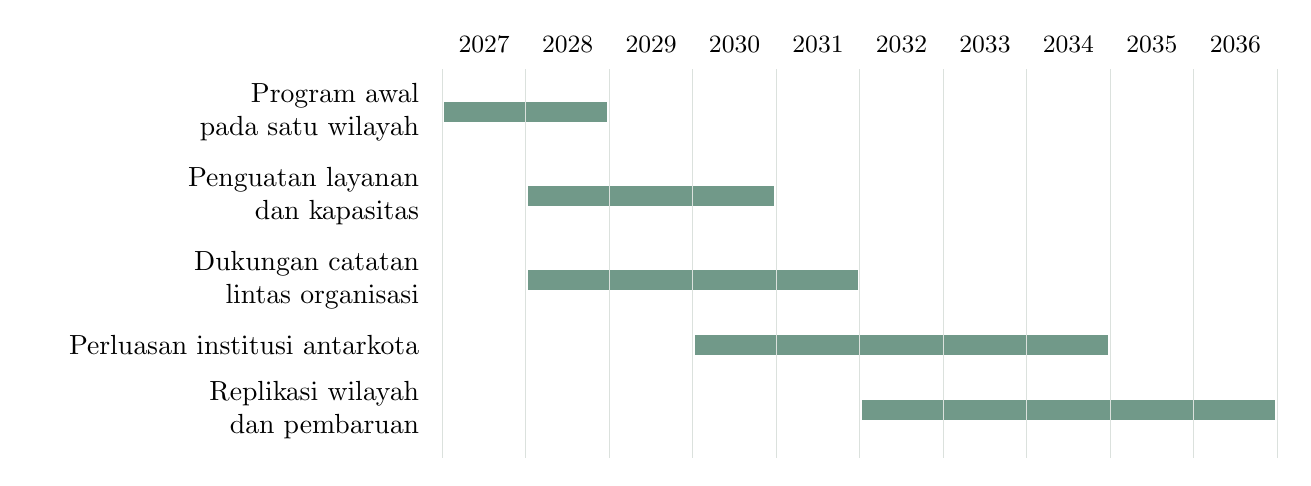
\begin{tikzpicture}[x=1cm,y=1cm]
\node[anchor=north east,text width=4.9cm,align=right,inner sep=2pt] (task0) at (-.22,0) {Program awal pada satu wilayah};
\coordinate (row0) at (0,0 |- task0.center);
\fill[forest!70] ($(row0)+(0.025,-.13)$) rectangle ($(row0)+(2.095,.13)$);
\node[anchor=north east,text width=4.9cm,align=right,inner sep=2pt] (task1) at ($(task0.south east)+(0,-.18)$) {Penguatan layanan dan kapasitas};
\coordinate (row1) at (0,0 |- task1.center);
\fill[forest!70] ($(row1)+(1.085,-.13)$) rectangle ($(row1)+(4.215,.13)$);
\node[anchor=north east,text width=4.9cm,align=right,inner sep=2pt] (task2) at ($(task1.south east)+(0,-.18)$) {Dukungan catatan lintas organisasi};
\coordinate (row2) at (0,0 |- task2.center);
\fill[forest!70] ($(row2)+(1.085,-.13)$) rectangle ($(row2)+(5.275,.13)$);
\node[anchor=north east,text width=4.9cm,align=right,inner sep=2pt] (task3) at ($(task2.south east)+(0,-.18)$) {Perluasan institusi antarkota};
\coordinate (row3) at (0,0 |- task3.center);
\fill[forest!70] ($(row3)+(3.205,-.13)$) rectangle ($(row3)+(8.455,.13)$);
\node[anchor=north east,text width=4.9cm,align=right,inner sep=2pt] (task4) at ($(task3.south east)+(0,-.18)$) {Replikasi wilayah dan pembaruan};
\coordinate (row4) at (0,0 |- task4.center);
\fill[forest!70] ($(row4)+(5.325000000000001,-.13)$) rectangle ($(row4)+(10.575000000000001,.13)$);
\coordinate (gridBottom) at ($(task4.south)+(0,-.16)$);
\node[font=\small,text width=0.9800000000000001cm,align=center,anchor=south] at (0.53,.18) {2027};
\draw[rule!50,line width=.3pt] (0.0,.1) -- (0.0,0 |- gridBottom);
\node[font=\small,text width=0.9800000000000001cm,align=center,anchor=south] at (1.59,.18) {2028};
\draw[rule!50,line width=.3pt] (1.06,.1) -- (1.06,0 |- gridBottom);
\node[font=\small,text width=0.9800000000000001cm,align=center,anchor=south] at (2.6500000000000004,.18) {2029};
\draw[rule!50,line width=.3pt] (2.12,.1) -- (2.12,0 |- gridBottom);
\node[font=\small,text width=0.9800000000000001cm,align=center,anchor=south] at (3.71,.18) {2030};
\draw[rule!50,line width=.3pt] (3.18,.1) -- (3.18,0 |- gridBottom);
\node[font=\small,text width=0.9800000000000001cm,align=center,anchor=south] at (4.7700000000000005,.18) {2031};
\draw[rule!50,line width=.3pt] (4.24,.1) -- (4.24,0 |- gridBottom);
\node[font=\small,text width=0.9800000000000001cm,align=center,anchor=south] at (5.83,.18) {2032};
\draw[rule!50,line width=.3pt] (5.300000000000001,.1) -- (5.300000000000001,0 |- gridBottom);
\node[font=\small,text width=0.9800000000000001cm,align=center,anchor=south] at (6.890000000000001,.18) {2033};
\draw[rule!50,line width=.3pt] (6.36,.1) -- (6.36,0 |- gridBottom);
\node[font=\small,text width=0.9800000000000001cm,align=center,anchor=south] at (7.95,.18) {2034};
\draw[rule!50,line width=.3pt] (7.42,.1) -- (7.42,0 |- gridBottom);
\node[font=\small,text width=0.9800000000000001cm,align=center,anchor=south] at (9.01,.18) {2035};
\draw[rule!50,line width=.3pt] (8.48,.1) -- (8.48,0 |- gridBottom);
\node[font=\small,text width=0.9800000000000001cm,align=center,anchor=south] at (10.07,.18) {2036};
\draw[rule!50,line width=.3pt] (9.540000000000001,.1) -- (9.540000000000001,0 |- gridBottom);
\draw[rule!50,line width=.3pt] (10.6,.1) -- (10.6,0 |- gridBottom);
\end{tikzpicture}
}

\end{document}
